\section{Floating point types}
\label{sec:(chap3):floats}

Floating point types refer to numbers with a floating decimal point. There are 4
floating point types, shown in the table below. The built-in floating point
types conform to IEEE 754 arithmetic, which means, for example, that
\token{f32} has 1 bit of sign, \token{8} bits of exponent, and \token{24} (23
explicit) bits of mantissa. The \token{fsize} type represents the largest
floating-point type that can be represented on the target architecture.

\begin{center}
  \begin{tabular}{|c|lll|}
    \hline
    type & size & exp & mantissa\\[0pt]
    \hline
    \hline
    \texttt{f32} & 32 & 8 & 24 (23 explicit)\\[0pt]
    \texttt{f64} & 64 & 11 & 53 (52 explicit)\\[0pt]
    \texttt{f80} & 80 & 16 & 64 (63 explicit)\\[0pt]
    \texttt{fsize} & arch & arch & arch\\[0pt]
    \hline
  \end{tabular}
\end{center}

\subsection{Literals}
\label{sec:orgfd9f825}

Floating point types can be written in three different forms, decimal,
scientific notation.

\begin{enumerate}
  \setlength\itemsep{-4pt}
\item Decimal, two decimal int literals separated by the token \token{.} (with
  no spaces in between). \token{1837.0289}. The decimal part can be omitted,
  which means it is equal to \token{0} (e.g. \token{10.} is valid, but not
  \token{.10}).

\item Scientific notation, similar to decimal notation, but ending with an
  exponent preceded by the letter \token{e} or \token{E}. \token{3.14e78 ==
    (3.14 * 10.0 \^\^ 78)}, which is ($3.14 \times 10^{78}$). A sign for the
  exponential part can be set after the letter \token{e} or \token{E} with the
  token \token{-} or \token{+}, e.g. \token{3.e-10}. There must be no spaces in
  the literal.

\item Hexadecimal notation, starting with \token{0x}, then two hexadecimal int
  literal separated by the \token{.} token, followed by the letter \token{p}
  or \token{P}, and ending with a decimal int literal representing the
  exponential part. The fractional part can be empty, in which case the letter
  \token{p} follows the \token{.} token. However, the \token{.} token and the
  \token{p} exponential part are mandatory. A sign for the exponential part can
  be set after the letter \token{p} or \token{P} with the token \token{-} or
  \token{+}. There can be no spaces in the literal. Unlike scientific notation,
  the exponential part is a power of \token{2} instead of \token{10}, e.g.
  \token{0xA.p4 == (10.0 * 2.0\^\^4)}.

\end{enumerate}

The three forms can also contain the token \token{\_} to split long literals
and make them easier to read (e.g. \token{124\_732.789\_281},
\token{0x1.FFFF\_FFFFp1023}, \token{3.14\_15\_92e3f}). There can be as many
\token{\_} as you like, they will just be removed during compilation. Literals
can end with a suffix to specify the type of the literal; \token{f} to define
\token{f32} literals, \token{d} to define \token{f64} (for \token{double}),
\token{l} for \token{f80} (for \token{long}) and \token{r} for
\token{fsize} (for \token{real}). Literals without a suffix are considered to
be of type \token{f64}. The literals \token{4.5e10f} and \token{0.8f},
\token{0x1.FFp10f} are of type \token{f32} and \token{4.5e10} and
\token{0.8}, \token{0x1.FFp10} are of type \token{f64}.

\subsection{Properties}
\label{sec:org52a5d6e}

Floating point properties can be accessed by using the \token{::} operator on a
type expression. The properties are as follows:

\begin{center}
  \begin{adjustbox}{max width=1.01\linewidth}
    \begin{threeparttable}
      \begin{tabular}{|l|ll|}
        \hline
        Name & Meaning & Type\\[0pt]
        \hline
        \hline
        \texttt{init} & The initial value - nan (Not a Number) & \texttt{typeof(x)}\\[0pt]
        \Xhline{0.001pt}
        \texttt{max} & The maximal finite value & \texttt{typeof(x)}\\
        & that this type can encode & \\[0pt]
        \Xhline{0.001pt}

        \texttt{min} & The minimal finite value & \texttt{typeof(x)}\\
        & that this type can encode & \\[0pt]
        \Xhline{0.001pt}

        \texttt{nan} & The value Not a Number & \texttt{typeof(x)}\\[0pt]
        \Xhline{0.001pt}
        \texttt{inf} & The value positive infinity & \texttt{typeof(x)}\\[0pt]
        \Xhline{0.001pt}
        \texttt{epsilon} & The smallest increment & \texttt{typeof(x)}\\
        & to the value 1 &\\[0pt]
        \Xhline{0.001pt}
        \texttt{dig} & The number of decimal digit of precision & \texttt{u32}\\[0pt]
        \Xhline{0.001pt}
        \texttt{mant\_dig} & Number of bits in the mantissa & \texttt{u32}\\[0pt]
        \Xhline{0.001pt}
        \texttt{max\_10\_exp} & The maximum value &  \texttt{i32} \\
        & such that \(10^{max\_10\_exp}\) is representable &\\[0pt]
        \Xhline{0.001pt}
        \texttt{max\_exp} & The maximum value & \texttt{i32}\\
        & such that \(2^{max\_exp-1}\) is representable & \\[0pt]
        \Xhline{0.001pt}
        \texttt{min\_10\_exp} & The minimum value & \texttt{i32}\\
        & such that \(10^{min\_10\_exp}\) is representable$^1$  & \\[0pt]
        \Xhline{0.001pt}
        \texttt{min\_exp} & The minimum value & \texttt{i32}\\
        & such that \(2^{min\_exp-1}\) is representable$^1$ & \\[0pt]
        \hline
        \texttt{typeid} & A string encoding the name of the type & \texttt{[c8]}\\[0pt]
        \hline
      \end{tabular}
      \begin{tablenotes}
      \item[1.] \small \textit{as a normalized value}
      \end{tablenotes}
    \end{threeparttable}
  \end{adjustbox}
\end{center}

\begin{figure}[t]
  \centering
  \scalebox{0.65}{
    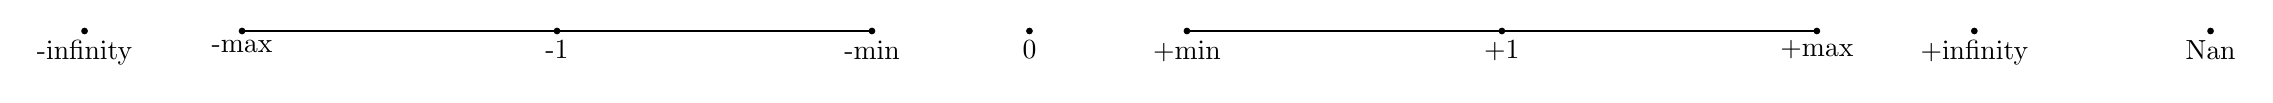
\begin{tikzpicture}
      \filldraw (0,0) circle (1pt) node[align=center, below] {-infinity};
      \filldraw (2,0) circle (1pt) node[align=center, below] {-max};
      \filldraw (6,0) circle (1pt) node[align=center, below] {-1};
      \filldraw (10,0) circle (1pt) node[align=center, below] {-min};
      \filldraw (12,0) circle (1pt) node[align=center, below] {0};
      \filldraw (14,0) circle (1pt) node[align=center, below] {+min};
      \filldraw (18,0) circle (1pt) node[align=center, below] {+1};
      \filldraw (22,0) circle (1pt) node[align=center, below] {+max};
      \filldraw (24,0) circle (1pt) node[align=center, below] {+infinity};
      \filldraw (27,0) circle (1pt) node[align=center, below] {Nan};

      \draw[-](2,0) -- (10, 0);
      \draw[-](14,0) -- (22, 0);

    \end{tikzpicture}
  }
  \caption{\label{fig:(chap3):float_point_size} Range of representable values with floating point types}
\end{figure}


\mycautionbox { The \texttt{min} value is not the opposite of the \texttt{max}
  value. Figure~\ref{fig:(chap3):float_point_size} describes the ordering relationship
  between values of floating-point types, where points and lines are the values
  that can be represented by a floating-point type. }

\subsection{Casting}
\label{sec:org9eacb07}

Floating point values can be cast to other types.

\begin{itemize}
  \setlength\itemsep{-4pt}
\item To other floating-point types: It is impossible to change the type of a
  float implicitly. The cast operator \token{cast!T (V)} can convert any float
  value to another float value of another float type. Because float values of
  different float types are coded with different numbers of bits, there may be
  stepping during casting.

\item To integer types: The cast operator can be used to convert a float value
  of any float type to an int value whose type is at least 4 bytes in size
  (\token{i32}, \token{u32} and larger). If the cast operator is used, the
  value is truncated to the floor value (e.g. \token{1.3} \token{1.5} and
  \token{1.8} are all truncated to \token{1}), and anything that was part of
  the decimal part of the float is lost. The reverse cast is also allowed (from
  any int type whose size is at least \token{4} bytes to any float type); in
  this case, some stepping may occur due to the floating-point encoding.

\end{itemize}

Floating point values cannot be converted to other types.
\subsubsection{Implicit casting}

The implicit casting of float values known at \token{cte} follows the same
rules as described for integer \token{cte} values.

\begin{lstlisting}[style=coloredverbatim, escapechar=@]
fn foo (f : f32) {}
fn foo (f : f64) {}

let a : f32 = 1.0; // ok, f64 is converted implicitely to f32

foo (1.0); // ok, using f64 definition
@\hb{foo (1.0r)}@; // error, both definitions work
\end{lstlisting}

\subsection{Unary operators}
\label{sec:org30770bf}

The \token{-} unary operators can be used on floating point types. The result
of the operation is the opposite value and is of the same type as the operand of
the operation. For example, \token{-89.0f} is of type \token{f32}.

\subsection{Binary operators}
\label{sec:orga43d13a}

Binary operators involving a float operand can only be used if both operands are
floats. There is an exception to this rule when the operation involves an object
operand that has overridden the said binary operator (as a left or right
operand). The binary operators are divided into 4 groups:

\begin{itemize}
  \setlength\itemsep{-4pt}
\item Arithmetic: Binary arithmetic operators can be used with two float values.
  The result of the operation takes the type of the largest operand (e.g. an
  operation with \token{f32} and \token{f64} takes the type \token{f64}). The
  operators that can be used are described in the table below.

  \begin{center}
    \begin{adjustbox}{max width=1.0\linewidth}
      \begin{tabular}{|c|lll|}
        \hline
        Operator & Operation & Commutative & Example\\[0pt]
        \hline
        \hline
        \texttt{+} & Addition & Yes & \texttt{1.0 + 2.3 == 3.3}\\[0pt]
        \texttt{-} & Subtraction & No & \texttt{1. - 8. == -7.}\\[0pt]
        \texttt{*} & Multiplication & Yes & \texttt{3. * 4. == 12.}\\[0pt]
        \texttt{/} & Division & No & \texttt{7. / 3. == 2.333}\\[0pt]
        \texttt{\%} & Rest of division & No & \texttt{7.23 \% 3.09 == 1.05}\\[0pt]
        \verb~^^~ & Exponant & No & \texttt{7.} \verb~^^~ \texttt{3 == 343.}\\[0pt]
        \hline
      \end{tabular}
    \end{adjustbox}
  \end{center}

  The power operator \token{\^\^} is a special
  operator that can take a float or an integer as its right operand. If both
  operands are floats, then they must be of exactly the same type, and the
  result value takes the type of the operands. If the right operand is an int
  value, then the result of the operation takes the type of the left operand.

\item Logical: Binary logical operators can be used with two float values. The
  largest type of the two operands is used to cast the value of the operand with
  the smallest type, to avoid too much stepping (although stepping may still
  occur). The result of the operation is always of type \token{bool}.

  \begin{center}
    \begin{adjustbox}{max width=1.0\linewidth}
      \begin{tabular}{|c|lll|}
        \hline
        Operator & Operation & Commutative & Example\\[0pt]
        \hline
        \hline
        \texttt{>} & Greater than & No & \texttt{(12. > 11.) == true}\\[0pt]
        \texttt{<} & Lower than & No & \texttt{(12. < 11.) == false}\\[0pt]
        \texttt{>=} & Greater or equal & No & \texttt{(14. >= 14.) == true}\\[0pt]
        \texttt{<=} & Lower or equal & No & \texttt{(11. <= 19.) == true}\\[0pt]
        \texttt{==} & Equal & Yes & \texttt{(10. == 10.) == true}\\[0pt]
        \texttt{!=} & Not equal & Yes & \texttt{(10. != 10.) == false}\\[0pt]
        \texttt{<=>} & Is congruent & Yes & \texttt{(10. <=> 10.) == true}\\[0pt]
        \texttt{<!>} & Is not congruent & Yes & \texttt{(10. <!> 10.) == false}\\[0pt]
        \hline
      \end{tabular}
    \end{adjustbox}
  \end{center}

   \token{<=>} and \token{<!>} are special floating point operators designed
   to evaluate the equality and inequality of left and right operands, taking
   into account the possibility of stepping. In other words, it uses the
   \token{::epsilon} value of the floating point type (of the largest operand)
   to evaluate whether the left operand is equal to the right operand delta the
   epsilon value. They also check for \token{nan} equality and inequality.
   These operators are of course less efficient than the equality and inequality
   operators, as they involve multiple instructions and possibly conditional
   jumps.

\item Affectation: The affectation operator \token{=} can be used when the two
  operands are of exactly the same float type. The left operand must be a
  mutable lvalue (e.g. a mutable variable, a slice access, etc.). The
  affectation operator can be mixed with an arithmetic operator (e.g.
  \token{+=}, \token{/=}, etc.). In this case, the operation \token{x += y}
  is rewritten as \token{x = x + (y)}, where the y operand always has a higher
  priority than the affectation operator. For example, the operation \token{x
    *= 12. + 3.} is rewritten as \token{x = x * (12. + 3.)}, even though the
  multiplication operator has a higher priority than the addition operator, i.e.
  the result of \token{x *= (12. + 3.)} is different from the result of
  \token{x = (x * 12. + 3.)}.

  \begin{lstlisting}[style=coloredverbatim]
let mut a = 11.0;
let b = a * 12.0 + 3.0;
a *= 12.0 + 3.0;

assert (b == 135.0);
assert (a == 165.0);
  \end{lstlisting}

\item Range: The range operator can be used on two float values of exactly the
  same type, creating a \token{range} value. The range type is a native
  compound type, which is described in the following chapter (see
  section~\ref{sec:range_type}).

  \begin{center}
    \begin{adjustbox}{max width=1.0\linewidth}
      \begin{tabular}{|l|lll|}
        \hline
        Operator & Operation & Example & Interval\\[0pt]
        \hline
        \hline
        \texttt{..} & Range operator not inclusive & \texttt{34.f .. 12.f} & \texttt{[34.f;12.f[}\\[0pt]
            \texttt{...} & Range operator inclusive & \texttt{5.f ... 89.f} & \texttt{[5.f;89.f]}\\[0pt]
            \hline
      \end{tabular}
    \end{adjustbox}
  \end{center}


  The value of the result range has a default increment of \token{1.0} and its
  inner type is the type of the operand. It can be ascending or descending
  depending on the values used to construct it.

\end{itemize}

\subsection{Overflowing and stepping}
\label{sec:orgd5d9f51}

Because of the way float values are encoded, there are gaps in the set of values
they can represent. Thus, some operations that should be mathematically
equivalent do not always produce the same float value. To compare two float
values, the property \token{::epsilon} can be used, as well as the congruent
operators \token{<=>} and \token{<!>}. There is no value overflow checking
at compile time or runtime.

\vfill%
\pagebreak
